\chapter{Introduction}


\section{Dataset Shift}


In the field of machine learning and predictive modeling, it is often assumed that data distributions remain static, meaning they do not change between the training and deployment phases of the model. However, in practice, this assumption is rarely satisfied: data distributions can undergo significant changes between the training and testing scenarios.

This phenomenon is known as \curlyquotes{\textbf{dataset shift}}\cite{shiftbook} and is closely related to another field of study, referred to by various terms such as \curlyquotes{\textbf{transfer learning}} or \curlyquotes{\textbf{inductive transfer}}. Transfer learning addresses the problem of how information can be drawn from a number of only partially related training scenarios and used to provide better predictions in one of those scenarios compared to using only that specific scenario. Therefore, dataset shift represents a more specific case: it deals with relating information in, typically, two closely related environments to improve prediction in one given the dataset in the other. Given this issue, it is crucial to develop an understanding of the suitability of particular models under such changing conditions, and it is necessary to consider whether a different predictive model should be employed.

Among the various forms of dataset shift, covariate shift, studied and described by Shimodaira\cite{SHIMODAIRA2000227}, is one of the most extensively researched. It encompasses situations where the distribution of the covariates, $P(X)$ changes, while the conditional relationship $P(Y \mid X)$, representing the relationship between the covariates $X$ and the target $Y$, remains unchanged. In this case, the typical values of the covariates observed during testing differ from those observed during training.

	
\subsection{Most common causes of dataset shift}
	
The two most common and well-studied causes of dataset shift are:

\begin{enumerate}
	\item Sample selection bias
	\item Non-stationary environments
\end{enumerate}

\textbf{Sample selection bias} occurs when there is a discrepancy in the data distribution due to the training data being obtained through a biased method, and therefore not reliably representing the real environment in which the classifier will be used (the test set). This bias is not necessarily a flaw of the algorithm or data management process but a systematic defect in the way the data is collected or labeled, causing a non-uniform selection of training examples from the population. This often leads to bias being introduced during training. Dataset shift resulting from sample selection bias is particularly relevant when dealing with imbalanced classification problems, as, in highly imbalanced domains, the minority class is especially sensitive to misclassification errors due to its typically low number of samples.

In real-world applications, data often is not stationary (in time or space). One of the most relevant \textbf{non-stationary} scenarios involves adversarial classification problems, such as spam filtering and network intrusion detection.
	

\section{Covariate Shift}

As previously mentioned, covariate shift is a specific type of dataset shift often encountered in machine learning. It occurs when the distribution of input data changes between the training environment and the operational environment, while the underlying relationship between the input and output remains unchanged. Mathematically, this can be defined as follows:

\textbf{Definition:} \textit{Covariate shift} occurs only in problems of the type $X \to Y$ and is characterized by:

$$
P_{\text{tra}}(Y \mid X) = P_{\text{tst}}(Y \mid X) \quad \text{and} \quad P_{\text{tra}}(X) \neq P_{\text{tst}}(X)
$$

where $P_{\text{tra}}$ and $P_{\text{tst}}$ represent the probability distributions in the training data and test data, respectively.  

Covariate shift can affect a wide range of machine learning models, regardless of the specific task. It commonly arises in scenarios where models are used to classify data or predict trends based on certain features. This issue is particularly relevant in diverse applications, including but not limited to:
	
	\begin{enumerate}
		\item Image categorization and facial recognition systems
		\item Speech recognition and translation software
		\item Diagnostic and screening tools in healthcare
	\end{enumerate}
	
For example, consider a model designed to distinguish between cats and dogs. Our training data might consist of images like those shown in Figure \ref{fig:cani-gatti-tr}.
	
	\begin{figure}[H]
		\centering
		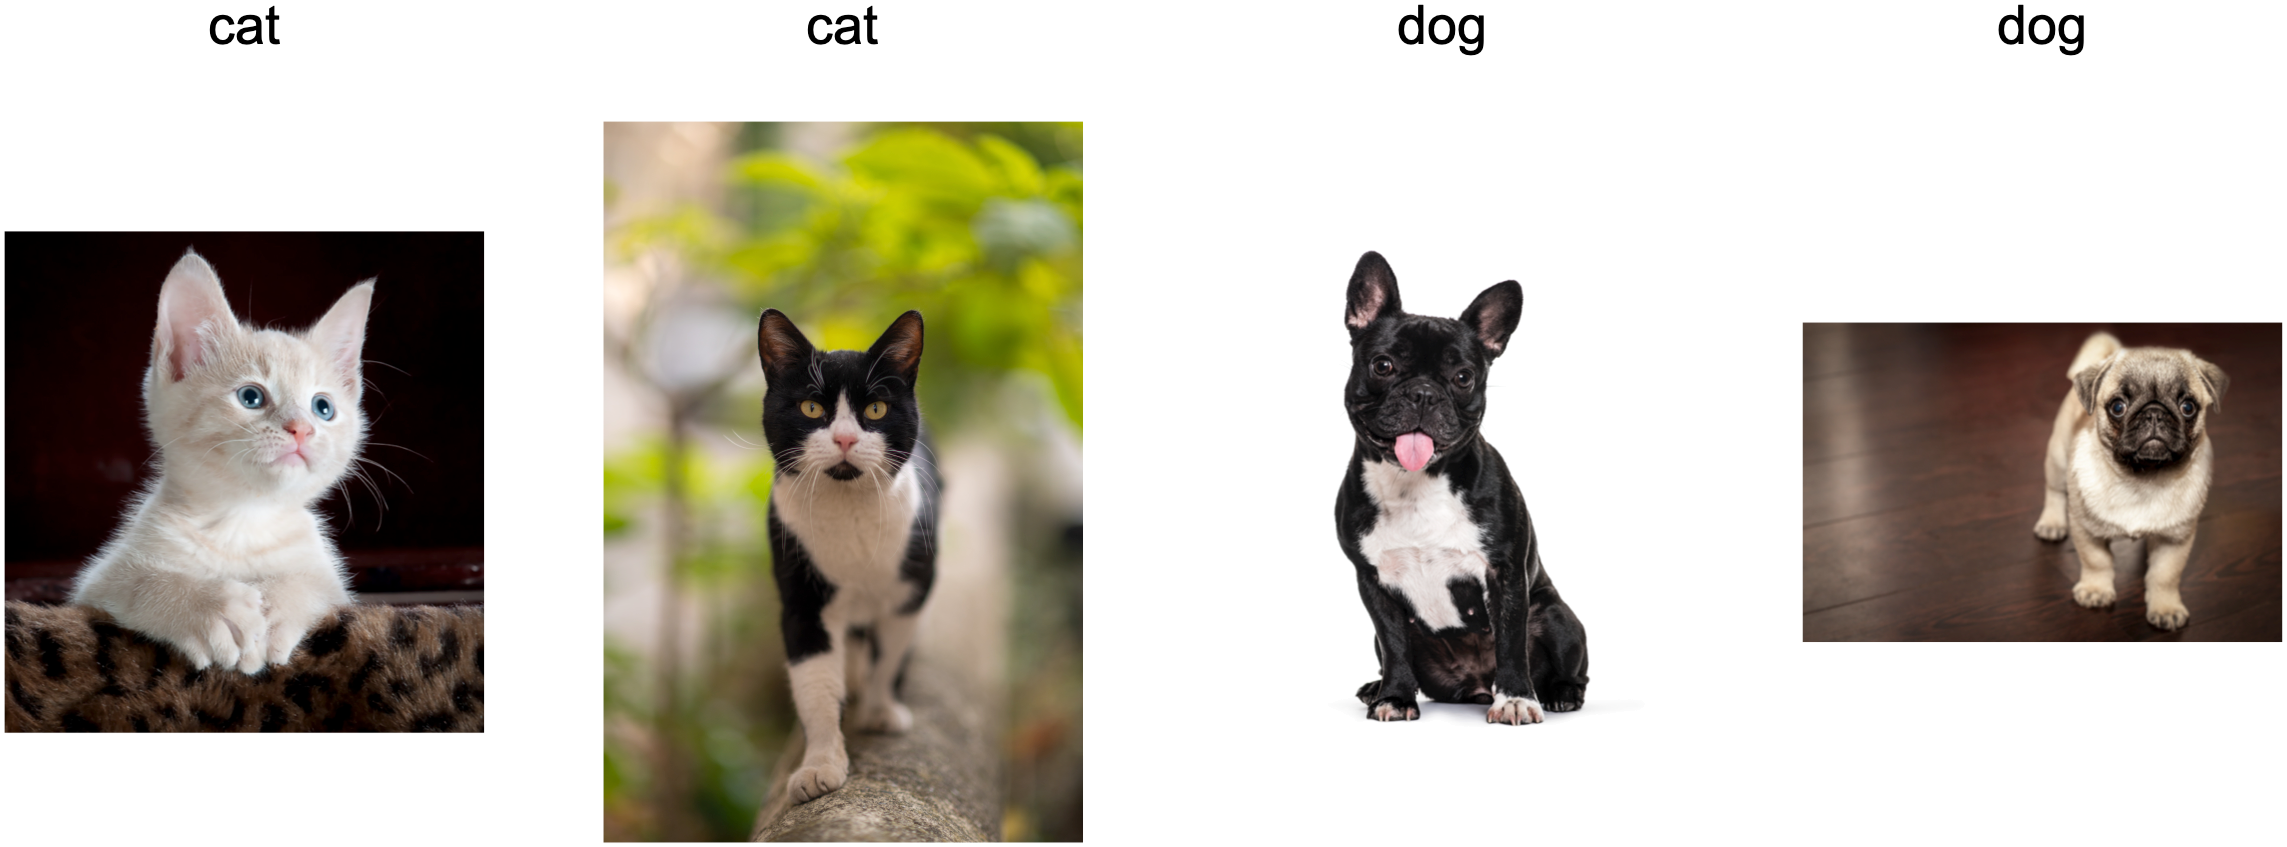
\includegraphics[width=1\textwidth]{assets/cat-dog-train.png} 
		\caption{Training data for distinguishing cats and dogs.}
		\label{fig:cani-gatti-tr}
	\end{figure}
     
At test time, we are asked to classify the images in Figure \ref{fig:cani-gatti-ts}, which have different characteristics. Because the feature distributions differ, the model may fail to accurately distinguish between cats and dogs once deployed.

Model may achieve a high degree of accuracy on a labeled training dataset, identifying and classifying the object in an image. 

However, when deployed with real-time data, changes in the input distribution can significantly impact the model's accuracy.
		
	\begin{figure}[H]
		\centering
		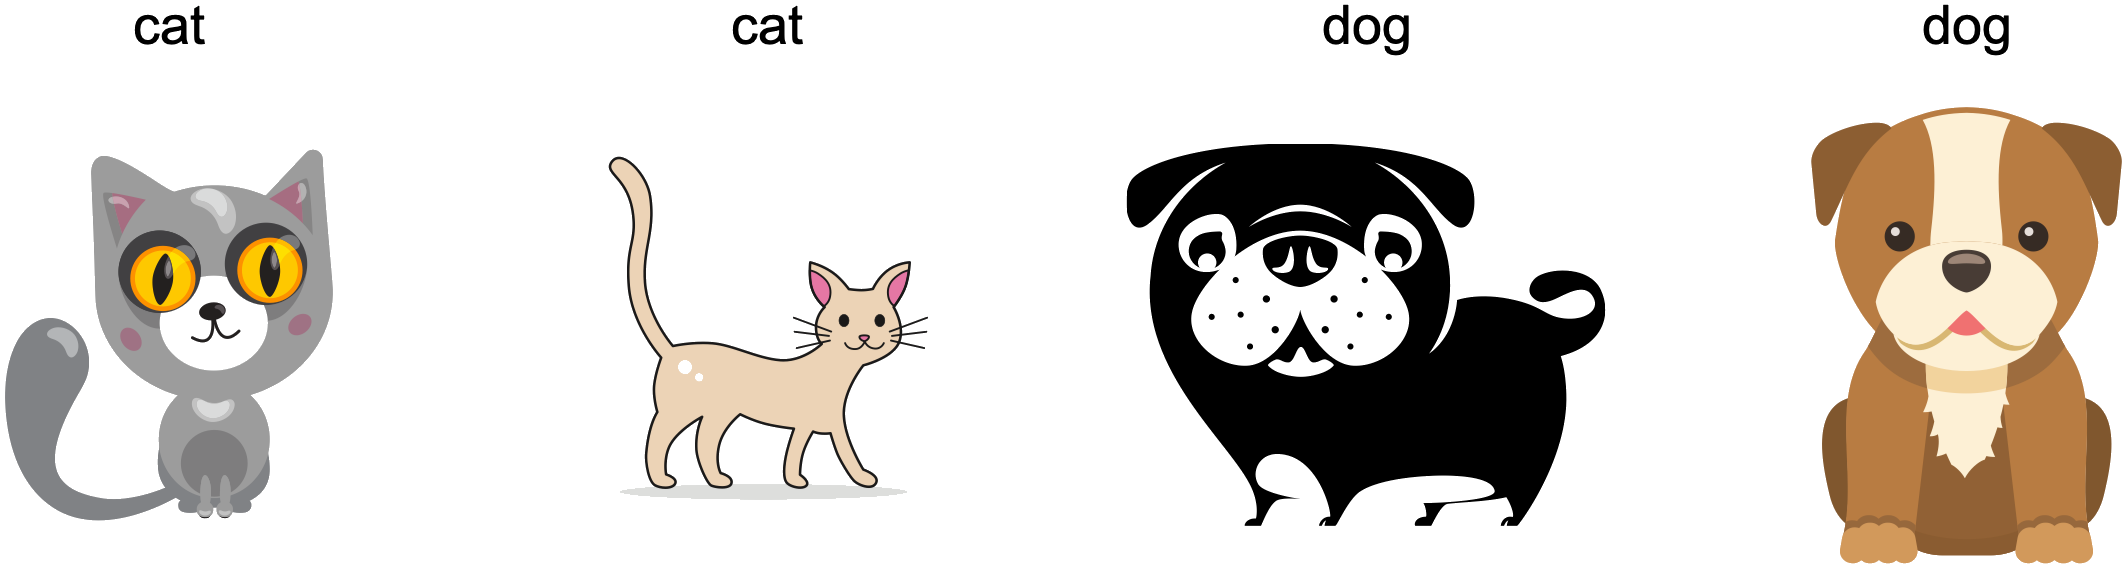
\includegraphics[width=1\textwidth]{assets/cat-dog-test.png} 
		\caption{Test data for distinguishing cats and dogs.}
		\label{fig:cani-gatti-ts}
	\end{figure}	
	
The same can happen in facial recognition systems. If the training data does not include individuals from certain ethnicities or age groups, the model may fail to generalize when deployed in an environment containing those unseen subpopulations. Similarly, changes in environmental conditions, such as lighting, can also contribute to covariate shift. For instance, a model trained under controlled lighting conditions may perform poorly when deployed in a setting with very different lighting.
	
Covariate shift, also known as \textit{covariate drift}, is thus a very common issue in machine learning. Supervised learning models are often trained with labeled data curated by data scientists who identify and analyze outliers to maintain high data quality. However, this level of oversight is not guaranteed in production environments, where the data can shift in ways the model was not prepared for. Thus, the training set may fail to perfectly mirror real-world conditions.

Figure \ref{fig:covariate-shift} shows an example of different distribution between training data and test data, creating a division between the two datasets.  

	\begin{figure}[H]
		\centering
		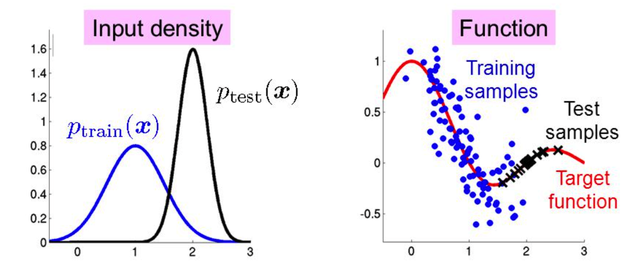
\includegraphics[width=0.8\textwidth]{assets/immagine.png} 
		\caption{Example of covariate shift.}
		\label{fig:covariate-shift}
	\end{figure}
	
This will have a negative impact on the accuracy of the model, as the algorithms will have been trained to map input data to output data and may fail to recognize the features of inputs from a different distribution, as shown in Figure \ref{fig:inaccurate-model}  
	
	\begin{figure}[H]
		\centering
		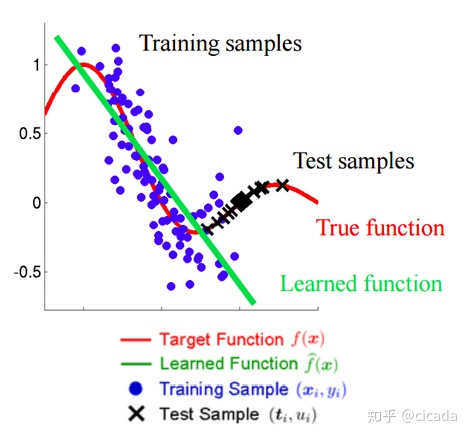
\includegraphics[width=0.5\textwidth]{assets/covariate_shift.png} 
		\caption{Example of inaccurate model.}
		\label{fig:inaccurate-model}
	\end{figure}  

This means that the model may become less accurate or even completely ineffective. A highly performant model on training data may not remain accurate once deployed. The goal is to measure the extent of the shift, take mitigating steps, and ultimately improve the model’s accuracy. Covariate shift can highlight the model’s generalization ability (i.e., how well it applies learned features to new data). Low generalization can result from overfitting, where the model aligns too closely with the training data, rendering it ineffective for new data drawn from a different distribution.